\documentclass[10pt,a4paper]{article}
\usepackage{polski}
\usepackage[utf8]{inputenc}
\usepackage{amsmath}
\usepackage{amsfonts}
\usepackage{amssymb}
\usepackage{courier}
%\renewcommand*\familydefault{\ttdefault} %% Only if the base font of the document is to be typewriter style
\usepackage[T1]{fontenc}
\fontsize{12}{15}
\usepackage[dvipsnames]{xcolor}
\definecolor{Mycolor2}{HTML}{FFFFED}
\pagecolor{Mycolor2}
\usepackage{tocloft}
\renewcommand{\cftsecleader}{\cftdotfill{\cftdotsep}}
%\color{RoyalBlue}
\renewcommand{\cftsecaftersnum}{.}
%fuksjowy
\colorlet{Fuksjowy}{RubineRed!70!}
\usepackage{secdot}
\usepackage{graphicx} % Required for the inclusion of images
\title{Burgundowi\protect \\ \hfill \newline \newline KCK 2017 -- Recenzja zadania drugiego\\ \newline\newline dla \textcolor{Fuksjowy}{Fuksjowych}\\ } % Title
\begin{document}
\maketitle  % Insert the title, author and date
\thispagestyle{empty}
\vfill
© \scriptsize{Copyright by Burgundowi (Michał Bronikowski i Radosław Madzia)}
\newpage
\tableofcontents
\newpage
\large
\section{Uwagi ogólne}
Uważamy, że macie słusznie rację i KSI rzeczywiście potrzebuje porządnej strony internetowej, jednak nie możemy zgodzić się z tym, że na obecnej stronie nie znajdziemy żadnych istotnych informacji na temat działalności koła.
\begin{center}
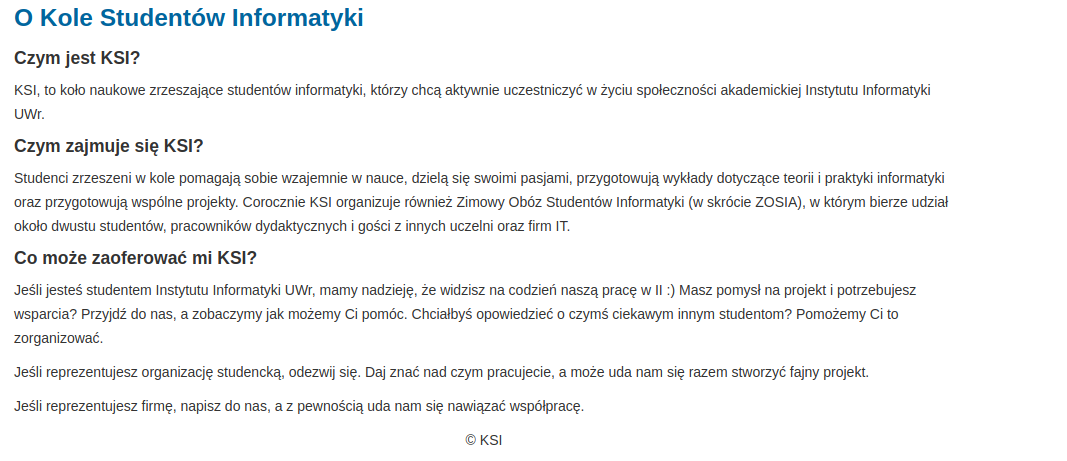
\includegraphics[width=\textwidth]{ksi}
\end{center}
Prawdą natomiast jest fakt, że na stronie nie znajdziemy żadnych informacji dotyczących rekrutacji do koła.
\section{Uwagi dotyczące zasięgniętych opinii}
Mamy zastrzeżenia do opisu opinii Łukasza Kostrzewskiego. Osoby czytające wasz dokument niekoniecznie muszą wiedzieć czym jest układ ,,pushrod”, a czytając o szanownym konstruktorze tego układu można odnieść wrażenie, że to on jest jego wynalazcą co po sprawdzeniu w internecie okazuje się nieprawdą. Uważamy więc, że takie przedstawienie jego osoby może być mylące. Koło Studenckie PWr Racing Team, niekoniecznie musi być znane dla studentów Informatyki UWr.
\section{Uwagi dotyczące postawionej diagnozy}
Podzielamy waszą opinię, jednak uważamy, że moglibyście podejść do tego tematu szerzej i lepiej go opisać(jedno zdanie to trochę mało).
\section{Uwagi dotyczące proponowanego rozwiązania}
Znowu uważamy, że podeszliście do tematu zbyt ogólnie. Moglibyście przynajmniej napisać czym wasz serwis będzie się różnił od poprzedniego, same zastosowanie najnowocześniejszych technologii niestety nie rozwiązuje naszego problemu.
\section{Kilka słów na zakończenie}
W pełni zgadzamy się z waszymi postulatami i z chęcią zobaczymy owoce waszej pracy. Życzymy wam dalszej owocnej pracy i mamy nadzieje, że nasze uwagi będą pomocą, a nie przeszkodą.\\ \\ Do zobaczenia na zajęciach :)
\end{document}